\subsection{$\Gamma_1 = \{2\}$, $\Gamma_2 = \{1\}$}
The initial quiver is illustrated in Figure~\ref{f:h_n=3_2-1}. 
\begin{figure}[htb]
\begin{center}
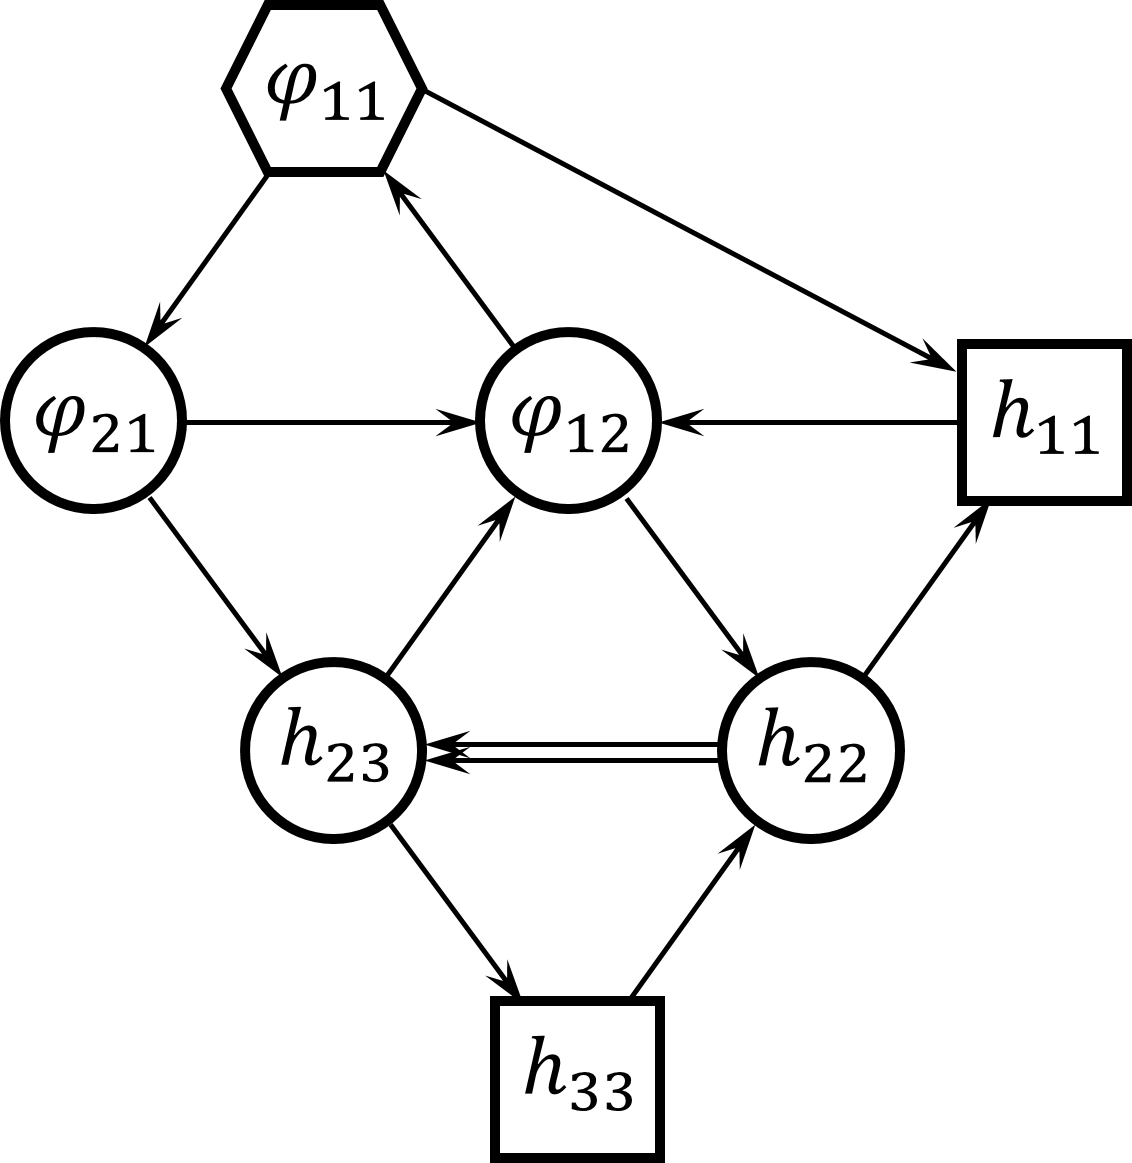
\includegraphics[scale=0.65]{h_convention/h_n=3_2-1.png}
\end{center}
\caption{The initial quiver for $\gc_h^{\dagger}(\bg,\GL_3)$ with $\Gamma_1 = \{2\}$, $\Gamma_2  = \{1\}$.}
\label{f:h_n=3_2-1}
\end{figure}

\paragraph{The initial variables.} All the variables in the initial extended cluster are as in $\gc_{h}^{\dagger}(\bg_{\std},\GL_3)$ except the variable $h_{33}$, which is given by
\begin{equation}
    h_{33}(U) = u_{33} \det U^{[2,3]}_{[2,3]} + u_{23} \det U_{[2,3]}^{\{1,3\}}.
\end{equation}

\paragraph{Birational quasi-isomorphisms.} The birational quasi-isomorphism \[\mathcal{Q}: (\GL_3,\gc_h^{\dagger}(\bg_{\std})) \dashrightarrow (\GL_3,\gc_h^{\dagger}(\bg))\]is given by
\begin{equation}
\mathcal{Q}(U)= (I-\alpha(U)e_{32})U(I+\alpha(U)e_{32}), \ \ \alpha(U):= \frac{\det U^{\{1,3\}}_{[2,3]}}{\det U^{[2,3]}_{[2,3]}}.
\end{equation}